% =============================================================================
% Section 4 — The POLE Refutation
% =============================================================================
\section{The \texttt{POLE} Refutation: When the Ceiling Broke}\label{sec:refutation}

\begin{objectives}
\begin{itemize}[leftmargin=*,itemsep=1pt,topsep=1pt]
  \item Read a mutation-rate table and extract the one comparison that tests a theory.
  \item Apply PSR$_2$ to real measurements and determine whether a model class survives.
  \item Distinguish refuting a \emph{parameterisation} from refuting a \emph{mechanism class}.
  \item Recognise why controls that cannot fail provide no evidence.
\end{itemize}
\end{objectives}

\subsection{Biological setting}

Somatic mutations in the proofreading domain of \texttt{POLE} produce some of the
most heavily mutated tumours in oncology. The most frequent is
\texttt{p.Pro286Arg} (\texttt{P286R}; dbSNP \texttt{rs1057519943}, ClinVar
\texttt{VCV000216066}), found in colorectal and endometrial carcinoma.

Residue $286$ sits inside the $3'\!\to\!5'$ exonuclease domain
(InterPro \texttt{IPR006133}), and this book does not take that on trust.
The boundaries are
retrieved live from InterPro and checked against the residue number by the
retrieval script \file{scripts/textbook/retrieve_genomic_data.py}, which refuses
to write its cache if the check fails. The domain spans residues $220$--$426$ of
the $2286$-residue protein, and $220 \le 286 \le 426$. The variant is where the
story says it is.

The natural hypothesis is therefore a stage-removal one: a lesion in the
proofreading domain removes proofreading. Section~\ref{sec:nogo} tells us exactly
what that hypothesis predicts, so we can test it.

\subsection{The experiment that decides it}

Human tumour data cannot test the hypothesis cleanly, because tumours differ in
too many other ways. What is needed is the yeast analogue, measured against an
exonuclease-null allele in the same genetic background.

Kane and Shcherbakova (2014) provide exactly that. In \emph{Saccharomyces
cerevisiae}, \texttt{pol2-P301R} is the structural analogue of human
\texttt{P286R}, and \texttt{pol2-4} is the catalytically dead exonuclease --- the
enzyme with proofreading entirely absent, which is to say $\kept = \emptyset$ and
$\errate = \inserr$. Both appear in the same table, measured on the same
\texttt{CAN1} forward-mutation reporter, in the same isogenic
mismatch-repair-proficient background:

\begin{table}[htbp]
\centering
\caption{Forward mutation rates at \texttt{CAN1} ($\times10^{-8}$), from Kane and
Shcherbakova (2014), Table~2. The final column is the quantity PSR$_2$ bounds.}
\label{tab:kane}
\begin{tabularx}{0.92\textwidth}{@{}l l r X@{}}
\toprule
\textbf{Allele} & \textbf{Proofreading} & \textbf{Rate} & \textbf{$\rho = $ rate / exo-null rate} \\
\midrule
wild type & intact & $1.5$ & $0.034$ \\
\texttt{pol2-4} & absent (exo-null) & $44$ & $1$ by definition --- this is $\inserr$ \\
\texttt{pol2-P301R} & domain mutated & $2300$ & $\mathbf{52.3}$ \\
\bottomrule
\end{tabularx}
\end{table}

\subsection{Applying the theorem}

PSR$_2$ says $\rho \le 1$ for every stage-removal mutant. The measurement gives
\begin{equation}\label{eq:rho}
  \rho \;=\; \frac{2300 \times 10^{-8}}{44 \times 10^{-8}} \;=\; \frac{2300}{44} \;\approx\; 52.3 .
\end{equation}
On the published $95\%$ confidence intervals the ratio is at least $35.3$. Either
way the bound is violated by more than an order of magnitude.

\begin{theorem}[Refutation]\label{thm:refuted}
The hypothesis that \texttt{P301R} acts by removing proofreading stages, in the
sense of Assumption~\ref{model:class}, is false.
\end{theorem}

\begin{proof}
Assumption~\ref{model:class} with Theorem~\ref{thm:psr2} implies $\rho \le 1$.
Equation~\eqref{eq:rho} gives $\rho \approx 52.3 > 1$. The hypothesis is
inconsistent with the measurement.
\end{proof}

\begin{remark}[A class, not a parameterisation]\label{rem:class}
It is worth dwelling on how strong this is. A measurement that disagreed with a
\emph{prediction} would ordinarily invite re-tuning: perhaps $\gamma$ was wrong,
perhaps there are more stages than we thought. None of that is available here.
Theorem~\ref{thm:psr2} holds for every $\gamma$ and every stage count
simultaneously, so there is no surviving member of the family to retreat to. The
mechanism class is excluded, not merely mis-parameterised.

Kane and Shcherbakova reached the same conclusion by a different route, and said
so in their title: \emph{fidelity defects distinct from loss of proofreading}.
The no-go theorem turns that qualitative judgement into a bound with a number
attached.
\end{remark}

\subsection{Controls}

A refutation is only as good as its controls. Three matter here.

\begin{enumerate}[leftmargin=*,itemsep=2pt]
  \item \textbf{Other cancer alleles.} \texttt{P286H}, \texttt{F367S} and
        \texttt{S459F} also exceed the ceiling (Barbari \emph{et al.}, 2018),
        so the failure is not a peculiarity of one substitution.
  \item \textbf{Neutral alleles.} \texttt{V411L} and six functionally neutral
        variants sit \emph{below} the ceiling and are not flagged. A test that
        flagged everything would be worthless.
  \item \textbf{The reference is not assumed.} $\inserr$ is not fitted; it is
        measured directly as the \texttt{pol2-4} rate in the same table. This is
        what makes $\rho$ a measurement rather than an estimate.
\end{enumerate}

\begin{figure}[htbp]
  \centering
  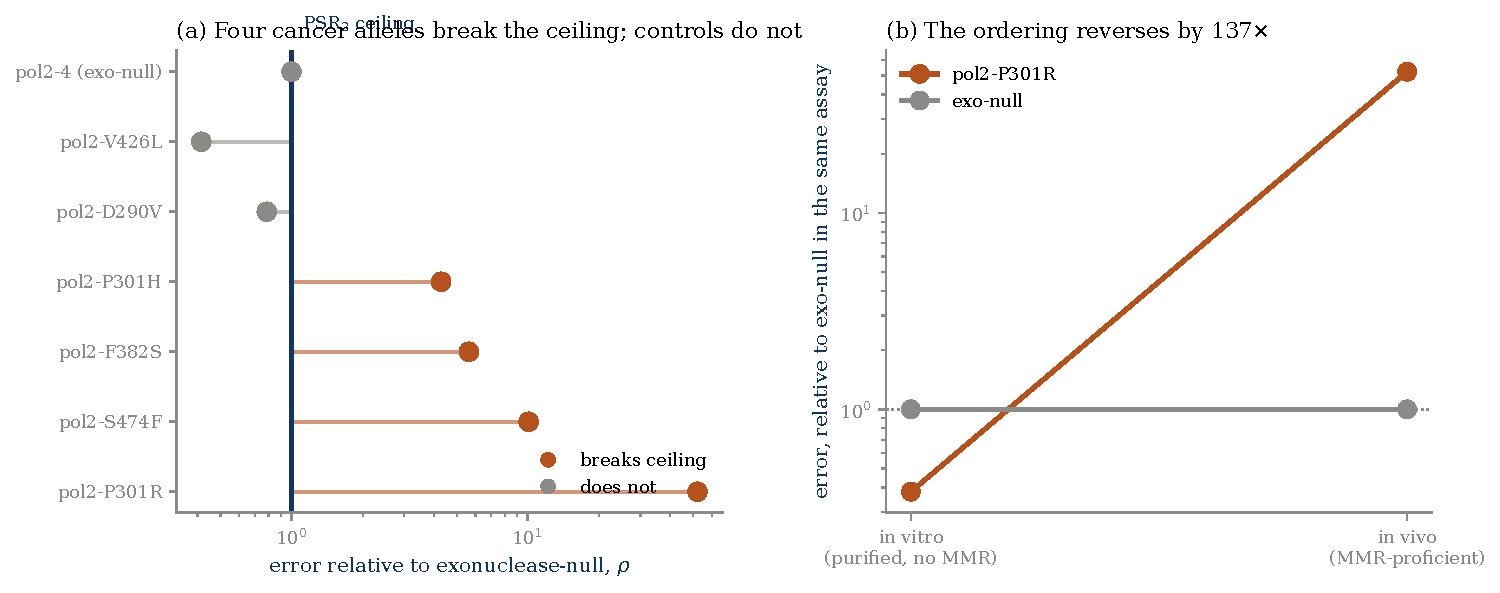
\includegraphics[width=\textwidth]{fig04_pole_panel.pdf}
  \caption{(a) The variant panel against the PSR$_2$ ceiling. Four
  cancer-associated alleles break it; the neutral control \texttt{V411L} and the
  exo-null reference do not. (b) The reversal that Section~\ref{sec:mmr} is built
  on: in a purified system \texttt{P301R} is \emph{more} accurate than exo-null,
  while in vivo it is $52\times$ worse. Between the test tube and the cell the
  ordering flips by a factor of $137$.}
  \label{fig:panel}
\end{figure}

\subsection{The clue in the reversal}

Refuting a mechanism leaves a question: if not stage removal, then what? The data
contain a sharp hint.

Xing \emph{et al.}\ (2019) purified the enzyme and measured its error rate with no
mismatch repair present. There, \texttt{P301R} makes $59 \times 10^{-6}$ base
substitutions against exonuclease-null's $155 \times 10^{-6}$. It is
\emph{more accurate} --- by a factor of about $2.6$ --- precisely where it was
supposed to be a catastrophe.

So the same pair of enzymes ranks one way in a tube and the opposite way in a
cell. Quantitatively, the ratio $\rho$ moves from $0.38$ in vitro to $52.3$ in
vivo, a reversal of $137$-fold.

\begin{remark}[What a reversal rules out]
A quantity that changes sign between two settings cannot be the variable that
explains the behaviour in both. Intrinsic error \emph{production} is therefore not
what makes this allele a mutator --- the purified measurement settles that.
Whatever carries the phenotype must be something present in the cell and absent
in the tube. Section~\ref{sec:mmr} shows that this reasoning can be made into a
theorem, and that the missing factor is forced to be an interaction with repair.
\end{remark}

\begin{worked}[4.1: why the wild-type comparison is the wrong one]
\textbf{Problem.} A reviewer objects: ``\texttt{P301R} is $2300/1.5 \approx 1533$
times wild type. Surely losing proofreading could produce that.'' Answer the
objection.

\textbf{Solution.} The objection compares against the wrong reference. Losing
proofreading \emph{can} produce a large ratio to wild type --- that is exactly
what \texttt{pol2-4} does, at $44/1.5 \approx 29$. The question PSR$_2$ asks is
different: can losing proofreading produce more errors than losing \emph{all} of
it? The answer is no, by Theorem~\ref{thm:psr2}, and the relevant ratio is
therefore $2300/44$, not $2300/1.5$.

The general lesson: a bound is only informative when you compare against the
quantity it bounds. Choosing a reference that makes a number look big is not the
same as testing a hypothesis. Worked Example~3.1 is the same error in its other
form.
\end{worked}

\begin{exercise}
Using PSR$_3$, compute the factor by which \texttt{pol2-P301R}'s insertion error
must exceed wild type's if one insists on keeping the stage-removal model.
Then explain, in one sentence, why the Xing measurement forbids that rescue.
\end{exercise}

\begin{exercise}
Suppose a new allele is measured at $\rho = 0.8$. Does this confirm the
stage-removal hypothesis for that allele? Say precisely what it does and does not
establish.
\end{exercise}

\begin{exercise}
Table~\ref{tab:kane} reports rates from a single reporter locus, \texttt{CAN1}.
Describe one way locus choice could bias $\rho$, and design a control that would
detect it.
\end{exercise}

\begin{exercise}[(harder)]
Edition~1 of this material presented a ``permutation test'' in which the
root-number labels of a dataset were shuffled and the test statistic recomputed.
The statistic turned out to be forced to its extreme value by a symmetry of the
pipeline. Explain why such a test yields a small $p$-value regardless of the data,
and state the general rule it violates.
\end{exercise}

\begin{ledger}
\textbf{Measured:} \texttt{CAN1} forward-mutation rates, Kane and Shcherbakova
(2014) Table~2: wild type $1.5$, \texttt{pol2-4} $44$, \texttt{pol2-P301R}
$2300$, all $\times10^{-8}$, same background and reporter. Purified-enzyme base
substitution rates, Xing \emph{et al.}\ (2019): $59$ versus $155 \times 10^{-6}$.
Additional alleles from Barbari \emph{et al.}\ (2018). Domain boundaries
\texttt{IPR006133} $= 220$--$426$ retrieved live from InterPro. \\
\textbf{Assumed:} that \texttt{pol2-P301R} is an adequate model of human
\texttt{P286R}, and that the \texttt{CAN1} reporter reflects genome-wide rates up
to a constant that cancels in $\rho$. \\
\textbf{Proved:} Theorem~\ref{thm:refuted}, by combining Theorem~\ref{thm:psr2}
with \eqref{eq:rho}. The arithmetic $2300/44 > 1$ needs no formalisation; the
bound it contradicts is machine-checked. \\
\textbf{Open:} what \emph{does} carry the phenotype. Section~\ref{sec:mmr}
narrows it; it does not finish the job.
\end{ledger}
